% !TeX TS-program = XeLaTex
% !TeX encoding = UTF-8
\documentclass[12pt]{beamer}
\usepackage{hyperref}
\usepackage[UTF8,noindent,fontset=]{ctex}
\usepackage{mathrsfs,tikz,xcolor,fontspec,graphicx,tcolorbox}
\usepackage{latexsym,amsmath,multicol,booktabs,calligra}
\usepackage{pstricks,listings,stackengine}
\usepackage{caption}
\usefonttheme[onlymath]{serif}
\usepackage[T1]{fontenc}
% \usepackage{concmath}
\usepackage{subfigure}
% \setCJKsansfont[ItalicFont=方正楷体_GBK.TTF]{方正苏新诗柳楷简体.TTF}
%\setCJKsansfont{方正宋刻本秀楷_GBK}
%\setCJKsansfont{Source Han Sans CN}
%\setCJKmainfont{Source Han Serif CN}
% \setCJKmainfont[BoldFont=方正小标宋_GBK.TTF]{方正新书宋_GBK.TTF}
\usepackage[orientation=landscape,size=custom,width=16,height=9,scale=0.5,debug]{beamerposter}
%修改比例
\usetikzlibrary{arrows.meta,bending}
\usetheme{Madrid}
\usecolortheme{beaver}
%页脚
\setbeamertemplate{footline}{
  \leavevmode%
  \hbox{%
    \begin{beamercolorbox}[wd=.333\paperwidth,ht=2.25ex,dp=1ex,center]{author in head/foot}
      \usebeamerfont{author in head/foot}\insertshortauthor
    \end{beamercolorbox}%
    \begin{beamercolorbox}[wd=.333\paperwidth,ht=2.25ex,dp=1ex,center]{title in head/foot}
      \usebeamerfont{title in head/foot}\insertshorttitle
    \end{beamercolorbox}%
    \begin{beamercolorbox}[wd=.333\paperwidth,ht=2.25ex,dp=1ex,right]{date in head/foot}
      \usebeamerfont{date in head/foot}\insertshortdate{}\hspace*{2em}
      \insertframenumber{} / \inserttotalframenumber\hspace*{2ex}
    \end{beamercolorbox}%
  }%
  \vskip0pt%
}
%\setbeamercolor{author in head/foot}{fg=white, bg=gray!100!black}  % 页脚作者颜色
%\setbeamercolor{title in head/foot}{fg=white, bg=gray!110!black}  % 页脚标题颜色
%\setbeamercolor{date in head/foot}{fg=white, bg=gray!120!black}  % 页脚日期颜色
%\title{我的演示文稿}
%\author{作者姓名}
\date[\today]{\footnotesize\today}
\AtBeginSection[]
{
	\begin{frame}{主要内容}
		\transfade%淡入淡出效果
		\tableofcontents[sectionstyle=show/shaded] %这几个参数我也不知道该如何准确地解释，反正它们最终的效果是突出显示当前章节，而其它章节都进行了淡化处理
		\addtocounter{framenumber}{-1}  %目录页不计算页码
	\end{frame}
}
% \definecolor{yaured}{cmyk}{0,1,1,0.45}
\definecolor{yaublue}{RGB}{0,112,192}
\definecolor{yaured}{RGB}{139,0,18}
\definecolor{uired}  {HTML}{db3f3d}
\definecolor{uiblue} {HTML}{4ea0b7}
\definecolor{uigreen}{HTML}{789a5b}
\definecolor{uigray} {gray}{0.95}
\definecolor{uilink} {HTML}{00769E}
\setbeamercolor{titlelike}{fg=yaured}
\setbeamercolor{structure}{fg=yaured}
\setbeamercolor{block body} {bg = uigray}
\setbeamercolor{block title}{fg = white,bg = yaured!80}
\setbeamercolor{caption name}{fg=yaured}
\setbeamercolor*{item projected}{fg=white, bg=yaured!80!white}

% 在右下角添加logo
% \logo{\includegraphics[width=2cm]{YAUWZ9.png}}
%\usetheme{cambridgeUS}
\title[1234]{延安大学\\延安大学中文beamer模板}
%多个作者及所属
\author{Zhen Wang\inst{1} \and Yijie Zhu\inst{2}}
\institute[123]{\small {\inst{1}School of Mathematics and Computer Science\and
 \inst{2} Affiliation of the 2nd author}}
  
\begin{document}
	\begin{frame}
		%\vspace{2cm}
		%\begin{center}
		%\resizebox{16em}{14pt}{\color{red!80} A brief introduction to Field-Feynman recursive model}\end{center}
		\begin{tikzpicture}[remember picture, overlay]
            \node[opacity=0.1] at ([shift={(0cm,-6.7cm)}]current page.north) {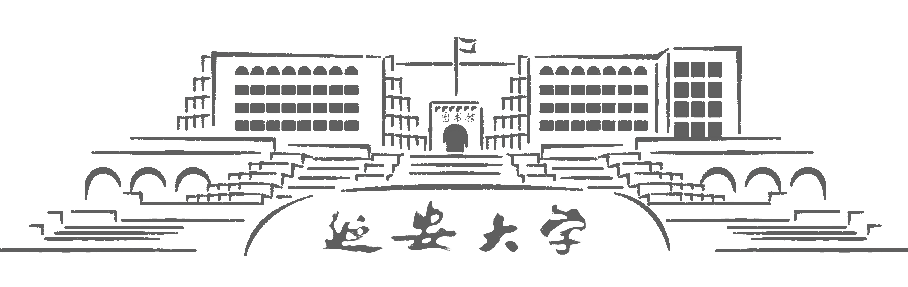
\includegraphics[width=14cm]{图一.png}};
        \end{tikzpicture}
		\titlepage
	\end{frame}
	
	% 在右上角添加logo
	\addtobeamertemplate{frametitle}{}{%
        \begin{tikzpicture}[remember picture,overlay]
        \node[anchor=north east,yshift=2pt] at (current page.north east) {
\includegraphics[height=0.9cm]{图二.png}};
        \end{tikzpicture}}
	
	\section{简介}
	\begin{frame}{简介}
			\begin{tikzpicture}[remember picture, overlay]
            \node[opacity=0.05] at ([shift={(4cm,-6.8cm)}]current page.north) {
\includegraphics[width=3.5cm]{图三.png}};
        \end{tikzpicture}
	    使用了Madrid主题。
	\end{frame}
	
	\section{插入公式及block}
	\begin{frame}{插入公式}
	    均值不等式
	    \[\frac{a+b}{2}\geqslant\sqrt{ab}.\]
	\end{frame}
	
	\begin{frame}{插入block}
	    \begin{block}{牛顿第一定律}
	        物体在不受外力时会保持匀速直线运动或静止。
	    \end{block}
	\end{frame}
	
	\section{插入图片}
	\begin{frame}{插入图片}
	    \begin{figure}
	        \centering
	        
\includegraphics[width=0.5\textwidth]{图四.png}
	        \caption{校徽 }
	        \label{fig1}
	    \end{figure}
	\end{frame}
	
	\beamertemplateshadingbackground{structure.fg!90}{structure.fg}
    \begin{frame}[plain]
    	\vfill
    	\centering
    	{
    		\centering \Huge \color{white}谢谢大家！
    	}
    	\vfill
    \end{frame}

\end{document}
